\section{Extended-Budget DDPM Validation}

To test whether higher ranks catch up with more optimization steps, we run a 20-epoch DDPM validation on ranks \(\{4,8,16\}\). Results are shown in Table~\ref{tab:extended_ddpm}.

\begin{table}[t]
  \centering
  \caption{Extended-budget DDPM validation (20 epochs, ranks 4/8/16).}
  \label{tab:extended_ddpm}
  \small
  \begin{tabular}{rrrrrrr}
    \toprule
    Rank & Trainable & Trainable(\%) & Runtime(s) & Peak MB & Final Loss & FID \\
    \midrule
    4  & 98304  & 0.0864 & 1045 & 2065.01 & 0.0407 & 130.8580 \\
    8  & 196608 & 0.1727 & 1044 & 2066.37 & 0.0343 & 132.2700 \\
    16 & 393216 & 0.3447 & 1040 & 2069.07 & 0.0311 & 131.3555 \\
    \bottomrule
  \end{tabular}
\end{table}

Compared with rank16 at 10 epochs (FID \num{132.2549}), rank16 at 20 epochs improves to \num{131.3555}. This is an absolute gain of \num{0.8994} and a relative improvement of approximately \num{0.6801}\%. The gain is measurable but modest, and does not reverse the broader moderate-rank preference under controlled budgets.

Figure~\ref{fig:ddpm_10_20} contrasts DDPM 10-epoch and 20-epoch behavior for ranks 4/8/16.

\begin{figure}[t]
  \centering
  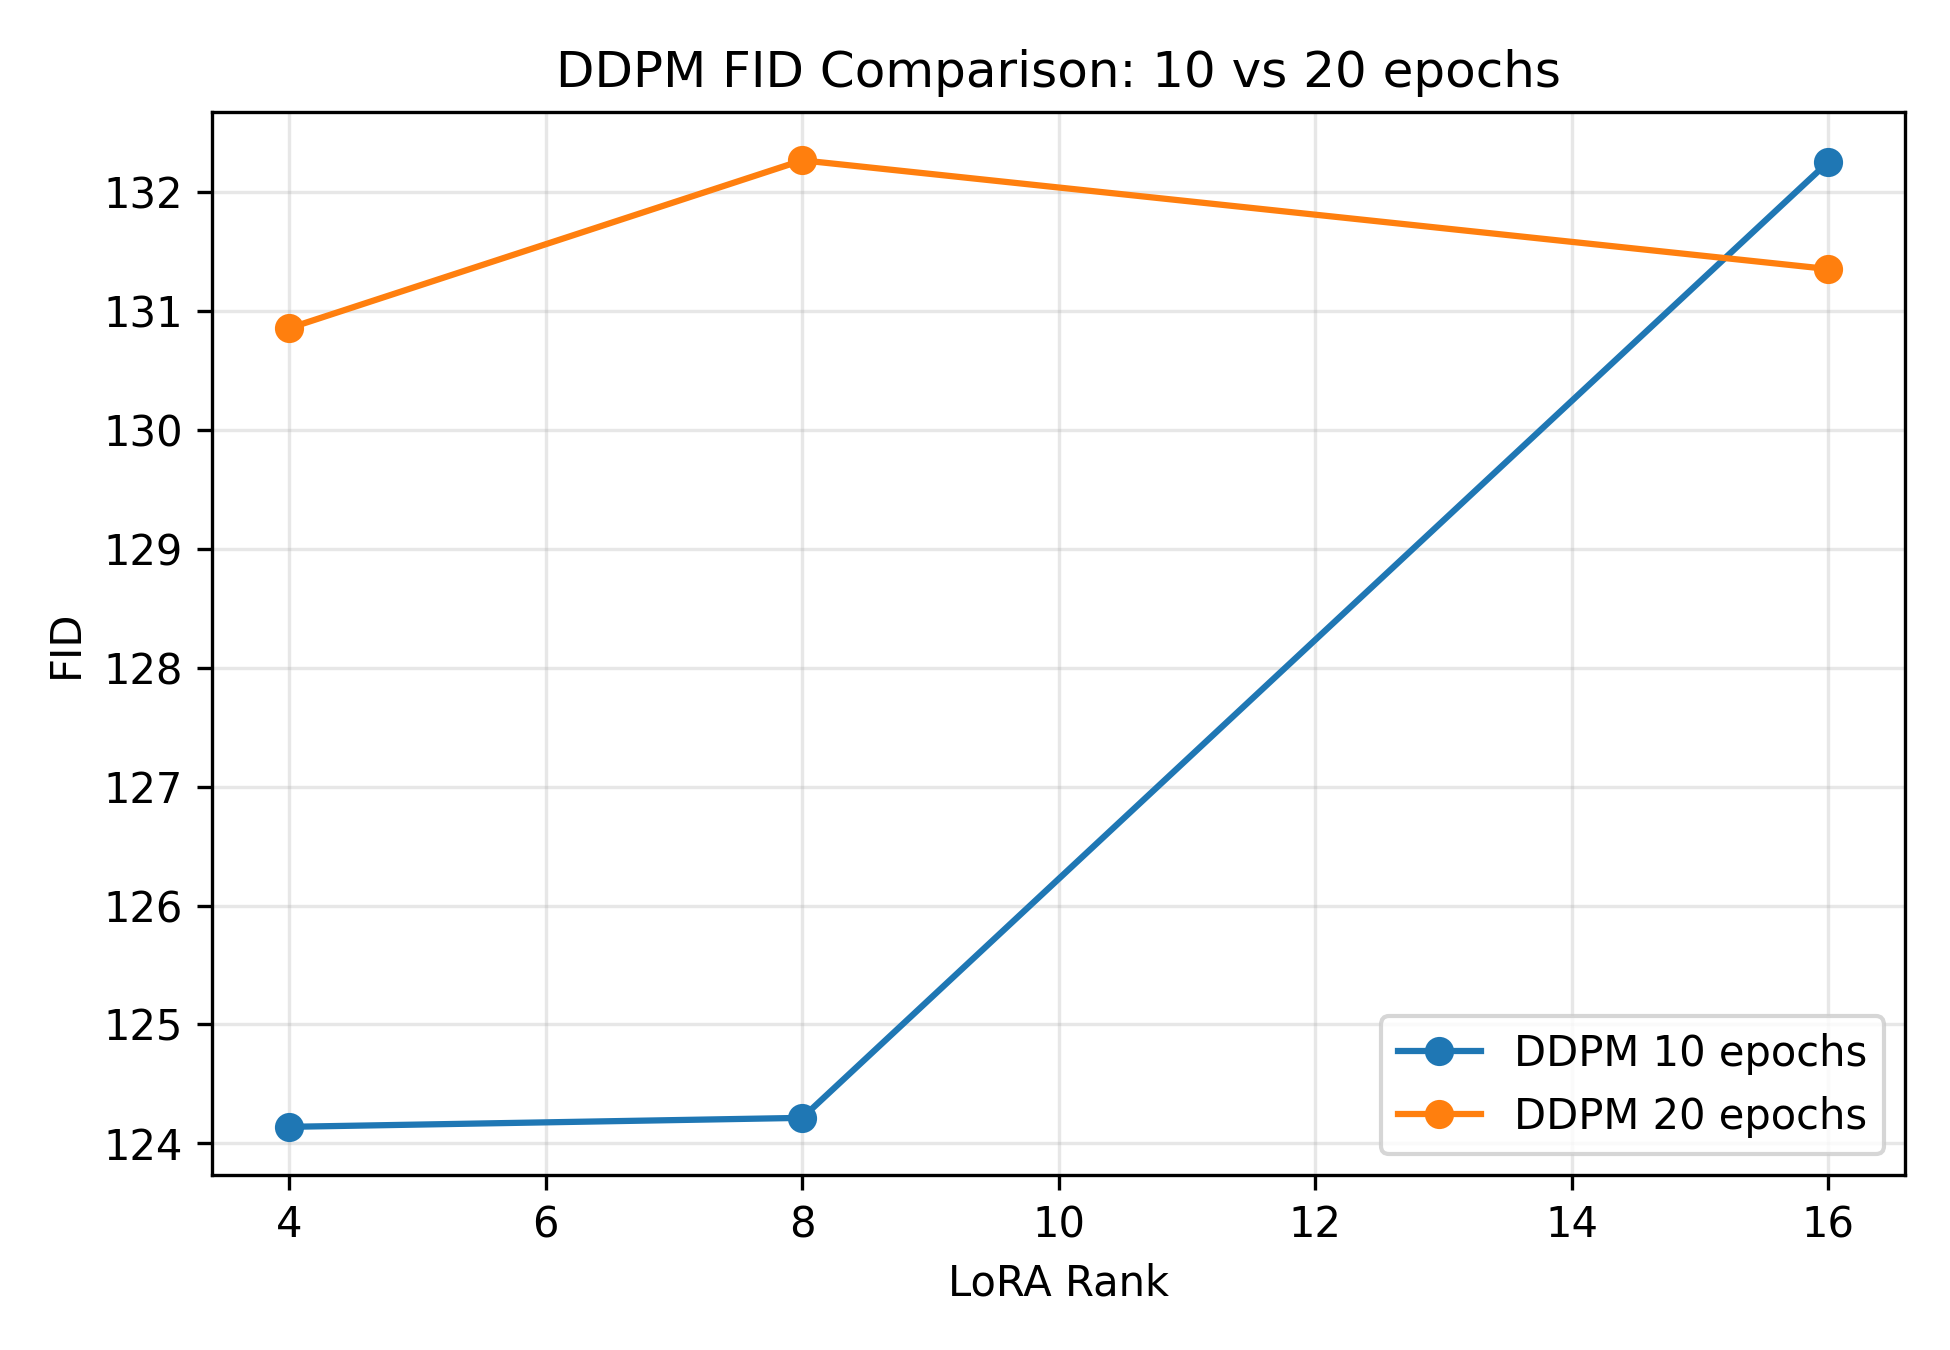
\includegraphics[width=0.9\linewidth]{../outputs/figures/ddpm_fid_10_vs_20_epoch.png}
  \caption{DDPM comparison at 10 vs. 20 epochs for ranks 4, 8, and 16.}
  \label{fig:ddpm_10_20}
\end{figure}
